\chapter{Background}

Databases
  PDB \citep{105}

GPU applications in bioinformatics
  sequence alignment \citep{123,1064}
  protein database search \citep{189}

Reviews
  anticancer drug development \citep{254}
  Ten Simple Rules for Getting Ahead as a Computational Biologist. Make software and website count \citep{260}

Early drug discovery
  Generalized Centroid Estimators in Bioinformatics \citep{272}

\section{Overview of the Pharmaceutical Industry}

Drug discovery is an industrial process. From 1950 to 2008, the US Food and Drug Administration (FDA) approved 1,222 new drugs \citep{717}. In 2008 and 2009, only 21 and 24 new drugs respectively were approved for marketing in the United States \citep{716}, well below the level required to secure the future of the pharmaceutical industry, which has been struggling with decreasing approval numbers for more than a decade. This is particularly remarkable because the level of investment in pharmaceutical research and development (R\&D) has dramatically increased by 12\% on average year-on-year since 1970 and at present to about US\$50 billion per year (Figure \ref{fig:NewDrugApprovals} \citep{686}).

\begin{figure}
\centering
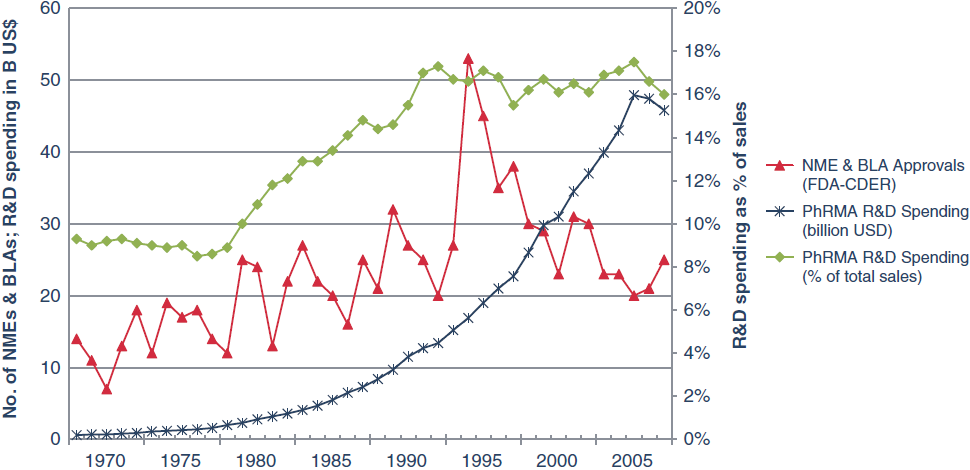
\includegraphics[width=\textwidth]{Background/NewDrugApprovals.png}
\caption{New drug approvals and R\&D investments by PhRMA-member companies from 1970 to 2009. Figure reprinted from \citep{686}.}
\label{fig:NewDrugApprovals}
\end{figure}

Drug discovery is an expensive and long-term business. A recent study in 2010 estimated that it takes US\$1.778 billion over a period of 13.5 years to develop a new drug (Figure \ref{fig:DrugDiscoveryProcess} \citep{716}). Broken down, the cost and cycle time broadly work out at US\$94 million and 1 year in hit identification, US\$166 million and 1.5 years in lead identification, US\$414 million and 2 years in lead optimization, US\$150 million and 1 year in preclinical phase, US\$273 million and 1.5 years in phase 1 clinical trials, US\$319 million and 2.5 years in phase 2 clinical trials, US\$314 million and 2.5 years in phase 3 clinical trials, and US\$48 million and 1.5 years in submission to launch.

\begin{figure}
\centering
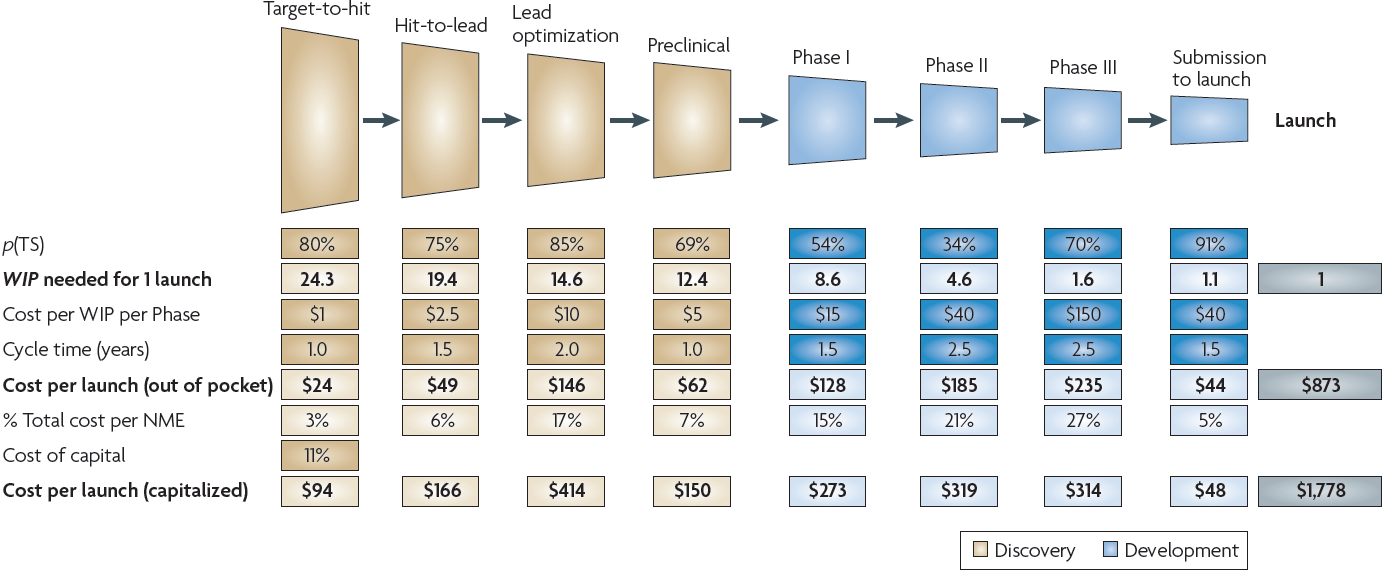
\includegraphics[width=\textwidth]{Background/DrugDiscoveryProcess.png}
\caption{R\&D model yielding costs and cycle times to successfully discover and develop a single new molecular entity (NME). Figure reprinted from \citep{716}.}
\label{fig:DrugDiscoveryProcess}
\end{figure}

Drug discovery is a high risk process and a wasteful game. It costs quite a lot to develop the ones that fail \citep{688}. It is estimated that for every 30,000 compounds synthesized, 2000 (6.7\%) enter preclinical development, 200 (0.67\%) enter phase 1 clinical trials, 40 (0.13\%) enter phase 2 clinical trials, 12 (0.04\%) enter phase 3 clinical trials, 8 (0.027\%) are approved, and 1 (0.003\%) makes a satisfactory Return On Investment (ROI) \citep{713}.

\section{The Process of Modern Drug Discovery}

How are drugs discovered and developed? This section paints a big picture for the state-of-the-art drug discovery process, and is organized according to the note entitled ``University of Survey'' by Dr. Steve Carney, the Managing Editor of Drug Discovery Today.

Figure \ref{fig:DrugDiscoveryProcess} \citep{716} shows the common steps that underpin drug discovery, including target identification, hit identification, lead identification, lead optimization, preclinical development, and clinical trials phases 1, 2 and 3.

\subsection{Development of an Innovative Idea}

All projects start with an idea, whose quality ultimately determines the value of a project. An idea is initiated from either an internal experiment, an external publication, or just the leisure moment in a bar. A drug discovery idea should link a process to a fundamental pathological pathway, altering which should be expected to be curative or antisymptomatic.

\subsection{Establishment of a Project Team}

In order to explore the potential of an innovative idea, one needs to populate a team. A team requires individuals with different expertise. Team members are typically made up of molecular biologists, \textit{in vitro} pharmacologists, automation specialists, medicinal chemists, process chemists, toxicology specialists, \textit{in vivo} pharmacologists, pathologists, bioinformaticians, chemoinformaticians, and the like. The importance of proper planning should never be underestimated.

\subsection{Target Discovery}

Once a team is established, the first task is to identify a biological target \citep{706,355,356,357,797}, which is any system that can potentially be modulated by a molecule to produce a beneficial effect.

A target is generally a protein (Figure \ref{fig:USAcademicDrugDiscoveryResearchFocus} \citep{721}), although it could be from a broad spectrum of moieties, be it a molecular entity (protein, gene, miRNA, fatty acid, carbohydrate, or lipid), a disease biomarker, a biological pathway, or a crucial node on a regulatory network, as long as it is relevant to a specific disease and its progression \citep{711}.

Pharmacology is essentially the science of the interaction of components foreign to the living body with components of the living body. Such foreign compounds interact with the human body through binding to a biological target molecule. As a result, the biological function of the target is altered such that a change in a pathway is induced. It is intended that this kind of modification of the pathway will produce a beneficial effect.

\subsection{Hit Identification}

Once a target is selected and validated, the next task is to identify hits, which are compounds that have activity at a predetermined level against a target, but little else is known at this early stage.

Hits are usually discovered by high throughput screening \citep{795,504,736} (Figure \ref{fig:USAcademicDrugDiscoveryResearchFocus} \citep{721}), which screens hundreds of thousands or even millions of compounds against the target in a high throughput manner. For the purpose of validation, discovered hits are re-screened against an alternative assay to rule out false positives.

\begin{figure}
\centering
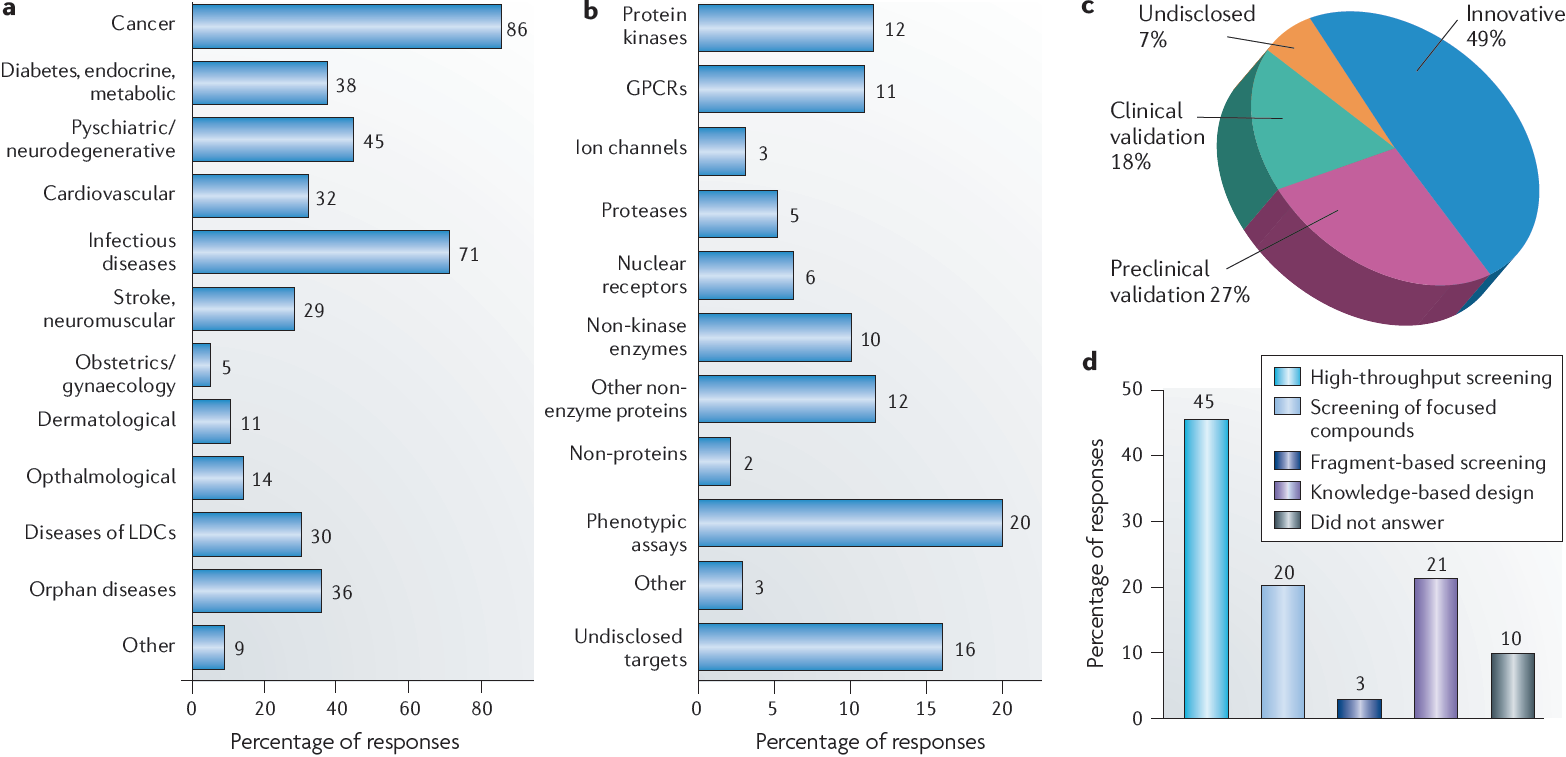
\includegraphics[width=\textwidth]{Background/USAcademicDrugDiscoveryResearchFocus.png}
\caption{Research focus of US academic and non-profit small-molecule drug discovery centres. (a) Therapeutic area. (b) Target-class focus. (c) Degree of validation of target portfolios. (d) Sources of tractable hits by discovery strategy. Figure reprinted from \citep{721}.}
\label{fig:USAcademicDrugDiscoveryResearchFocus}
\end{figure}

\subsection{Lead Identification}

Apart from just activity against the target, the next task is to identify those validated hits having properties that would indicate they have potential for being developed as drugs. A lead is a validated hit with several necessary properties, such as selectivity versus a panel of other targets, physicochemical characteristics, drug-like properties, and absorption, distribution, metabolism, excretion and toxicity (ADMET) properties. Only those molecules with acceptable potency, physical and ADMET properties can be advanced through lead optimization.

\subsection{Lead Optimization}

At this stage, medicinal chemists conduct extensive Structure-Activity Relationships (SARs) \citep{328} or use other methods \citep{661,475} to improve potency and selectivity, as well as physicochemical and drug-like properties. The optimized molecules are advanced to animal models and preliminary toxicology. They are scrutinised for potency, selectivity, bioavailability, safety, and massive productivity at a low price.

\subsection{Clinical Trials}

Immediately after lead optimization, the data on the successful candidates will then be submitted to the appropriate health authorities to get permission to conduct clinical investigations.

Compounds enter clinical trial at phase 1, which is focused on safety, tolerability and bioavailability rather than efficacy. The drug is administered to a small number of healthy volunteers.

Phase 2 clinical trials are focused on determining the efficacy of the drug in several hundred patients. These trials may be performed globally and give information on efficacy and allow for a further estimation of safety in a larger population.

Assuming satisfactory results from phase 2 studies, the drug will enter phase 3 clinical trials, which are in essence larger versions of the previous trials intended to answer specific questions with respect to efficacy. The trials would routinely involve several thousand patients and compare with drugs that are currently in use for the treatment of the disease. The results from these trials essentially form the basis of the risk/benefit analysis that will be submitted to the regulatory authorities.

Phase 4 clinical trials are often referred to as post-marketing studies and are performed after the medicine has been approved. These trials give a greater idea of long-term risk and benefit. The trials may involve many thousands of patients and go on for many years. Such trials may assist in indicating other uses for the medicine.

\section{Computational Drug Discovery}

Drug discovery via merely biological and chemical means are both cost-inefficient and time-inefficient. A computational framework for fast and accurate drug discovery is thus highly appreciated. The thesis concentrates on building computer models to simulate the three early stages of modern drug discovery process, namely hit identification, lead identification and lead optimization. From the computational perspective, they typically involve binding site identification, structure-based virtual screening, computational synthesis of potent ligands, drug properties prediction, interactive visualization, and so on. The thesis addresses structure-based virtual screening and computational synthesis of potent ligands.

Meanwhile, general-purpose computing on Graphics Processing Unit (GPU) is gaining more and more popularity in computationally intensive fields such as drug discovery.

\subsection{Structure-Based Virtual Screening}

As the X-ray crystallography and Nuclear Magnetic Resonance (NMR) technologies evolve, more and more 3D structures of biological macromolecules at atomic level have been revealed and deposited into the world's largest repository PDB (Protein Data Bank) \citep{540,539,537,105,538}. This rapid evolution catalyzes the development of various algorithms and tools for structure-based drug discovery via protein-ligand docking.

Protein-ligand docking is a method which predicts the preferred conformation (i.e. position and orientation) of a small ligand when bound to a macro protein to form a stable complex (Figure \ref{fig:Docking}, reprinted from Wikipedia). It also predicts the binding affinity in terms of free energy, which is basically the overall effect of various chemical forces involved, such as van der Waals force, electrostatic force, hydrogen bonding, hydrophobic interactions, Pi-Pi interactions, and the like. Free energy measures the degree of freedom of the ligand to ``escape'' from the protein, so the lower the free energy, the higher the binding affinity. Very often, the target protein is a viral enzyme of interest, and the small organic ligands that are predicted to inhibit the viral enzyme are what we want to discover.

\begin{figure}[t]
\centering
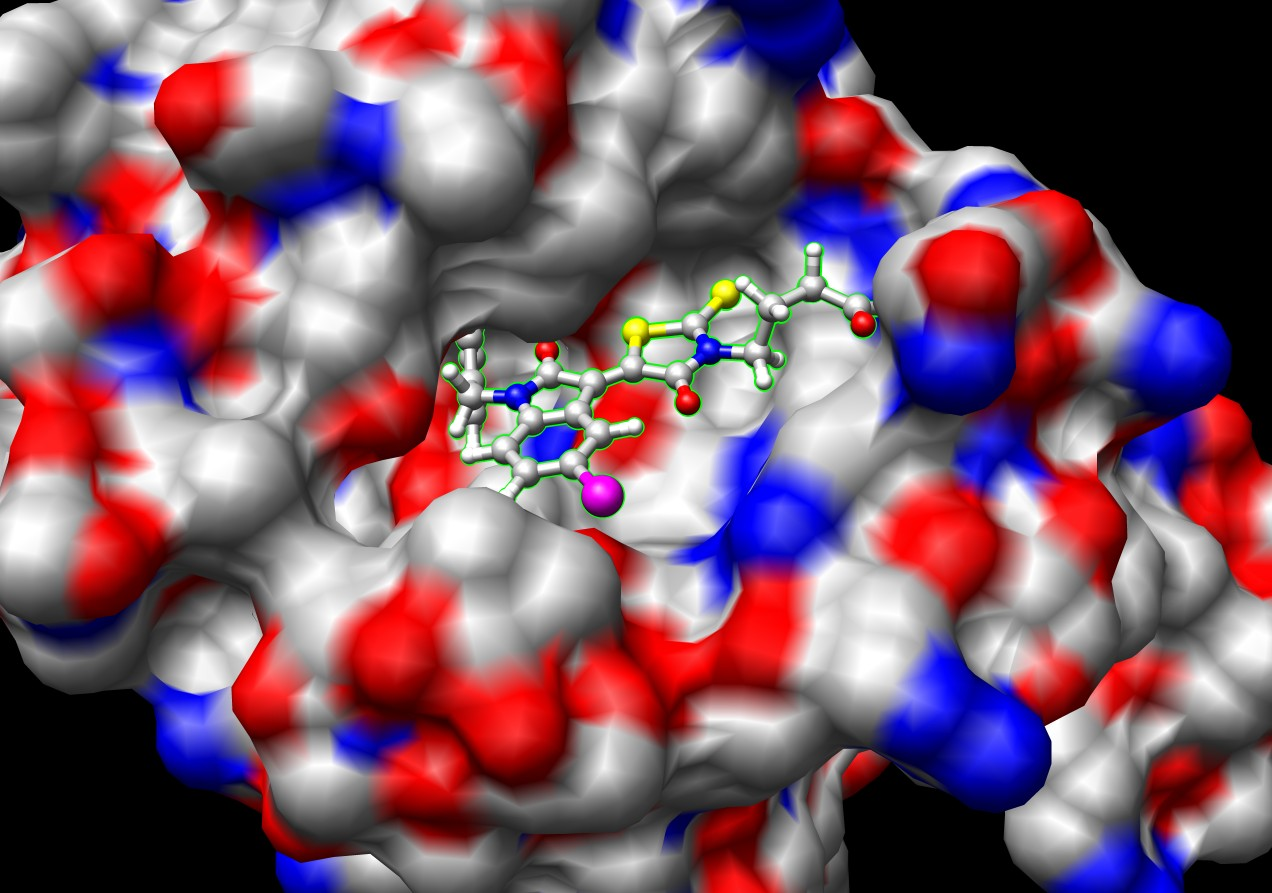
\includegraphics[width=\textwidth]{Background/Docking.jpg}
\caption{A ligand docked against a protein. Figure reprinted from Wikipedia.}
\label{fig:Docking}
\end{figure}

Docking programs typically consist of two basic components, a scoring function to predict the binding affinity, and an algorithm to explore the conformational space of the ligand and the protein \citep{493}. So far, dozens of scoring functions \citep{579,566,570,775,575,576,578,580,581,774} and dozens of algorithms \citep{595,564,594,602,603,604,605,606,607,781,614,615,617} have been developed. Some methods have been comprehensively evaluated and compared \citep{637,771,556}.

Among the many docking programs, AutoDock Vina \citep{595} (hereafter Vina for short) is a competitive one. It's free and open source. It runs faster than its predecessor AutoDock4 \citep{596} by an order of magnitude \citep{556}. Released in 2010, Vina has been cited by 117 other publications and adopted by many researchers \citep{609}. Indeed, it is intensively used in our research projects too.

Virtual screening is simply a massive version of docking (Figure \ref{fig:VirtualScreening} \citep{470}). It docks a database of drug-like ligands to a viral protein of interest, ranks them according to their predicted binding affinity, and shortlists the best ones for further investigation. Statistical frameworks and assessments have been established for evaluation and result selection \citep{489,491,769,583,582}. In reality, docking and virtual screening have successful applications for drug discovery \citep{495,498,751,503,752,757,506,738,761,763,766,736}.

\begin{figure}
\centering
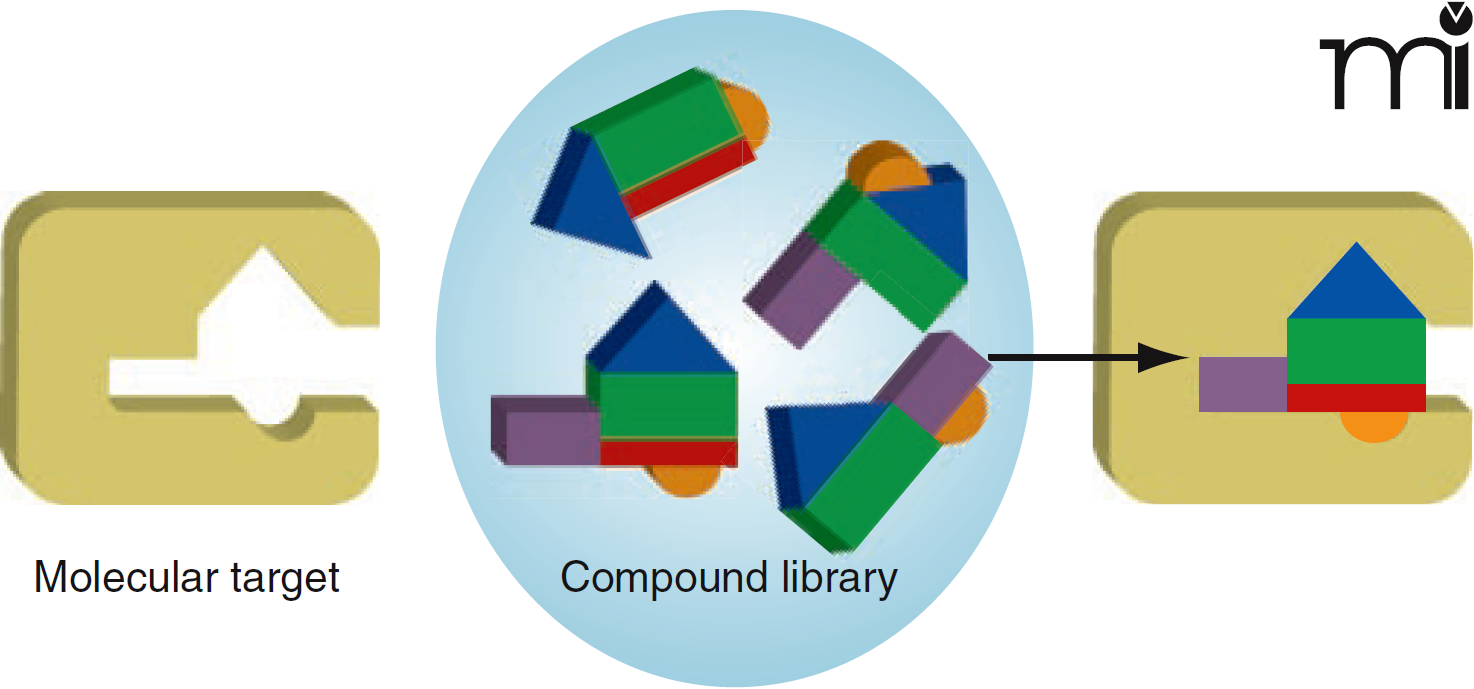
\includegraphics[width=\textwidth]{Background/VirtualScreening.png}
\caption{Virtual screening to identify compounds that bind to the target. Figure reprinted from \citep{470}.}
\label{fig:VirtualScreening}
\end{figure}

There are quite a lot data sources and databases for virtual screening, such as PDB \citep{540,539,537,105,538}, ZINC \citep{532}, PDBbind \citep{529,530}, and PubChem \citep{526}. In addition to raw data, there are library analysis \citep{521}, benchmark datasets \citep{534,533,535,536}, and data mainipulation tools \citep{542}. Some tools exploit massive parallelism in the form of either cluster computing or cloud computing \citep{557,773,560,782}.

\subsection{Computational Synthesis of Potent Ligands}

Virtual screening tries to discover promising ligands out of a database. Apparently the diversity of its outcome is limited to the diversity of the database. In other words, if the database contains no promising ligands at all, virtual screening will not succeed.

In contrast, computational synthesis produces novel molecular structures with desired pharmacological properties from scratch. Figure \ref{fig:ComputationalSynthesis} shows the relationship between synthesis and docking. Figure \ref{fig:LigandDesign} \citep{363} illustrates three kinds of strategies for ligand design. A number of compounds that evolved from fragments have entered the clinic, and the approach is increasingly accepted as an additional route to identifying new hits in inhibitor design \citep{363,470}.

\begin{figure}
\centering
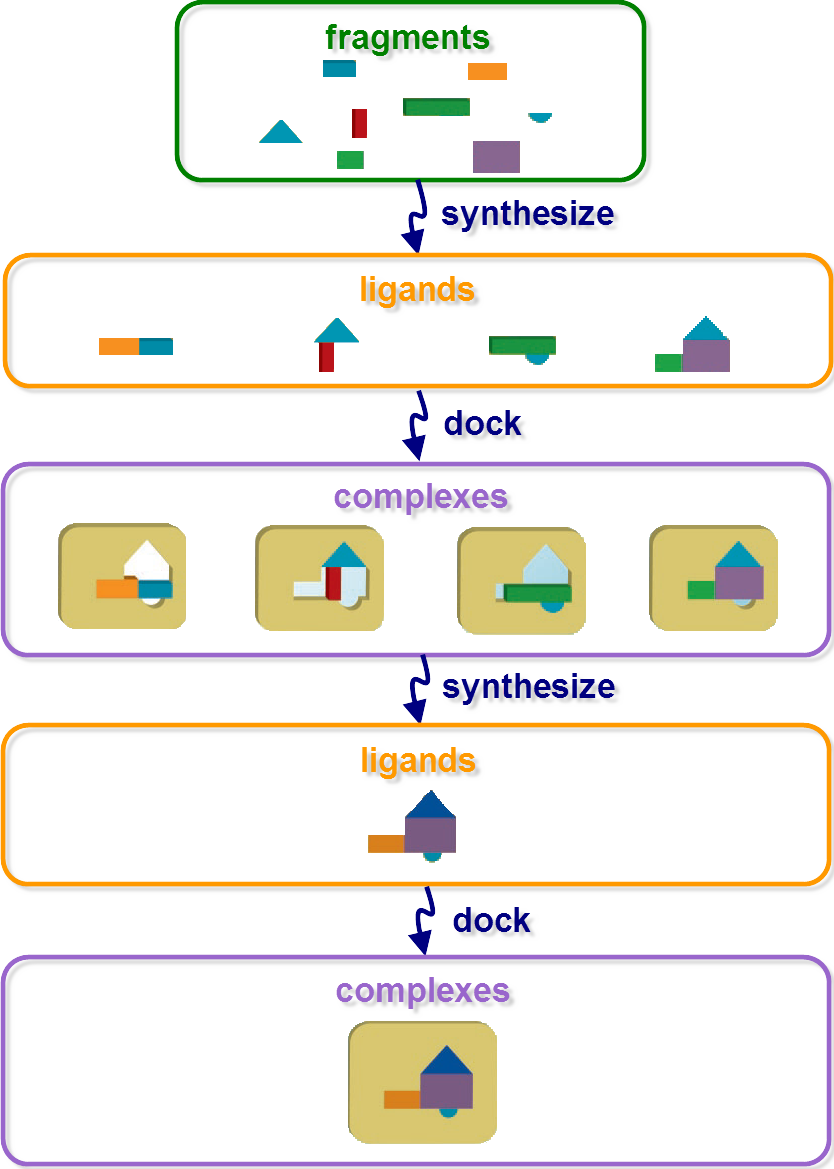
\includegraphics[width=\textwidth]{igrow/ComputationalSynthesis.png}
\caption{Synthesizing ligands from fragments followed by docking.}
\label{fig:ComputationalSynthesis}
\end{figure}

\begin{figure}[t]
\centering
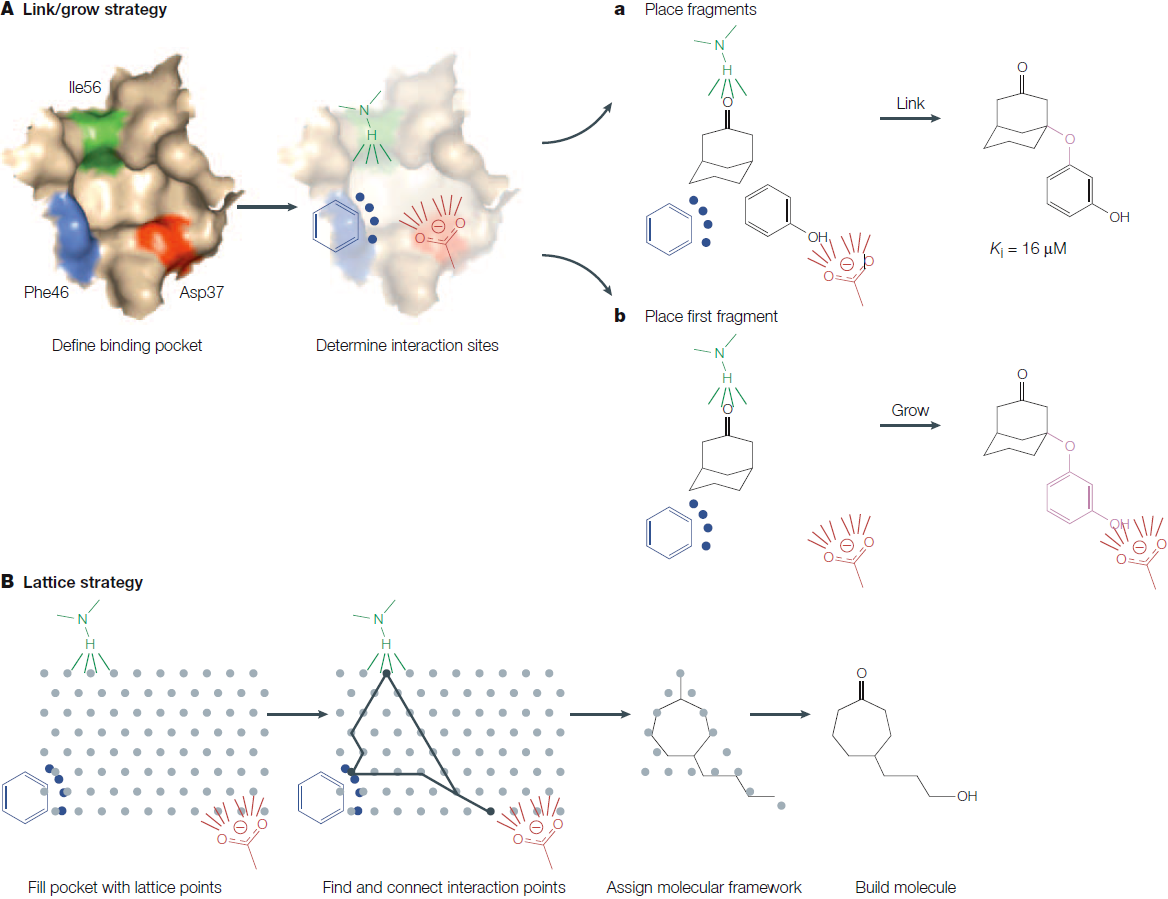
\includegraphics[width=\textwidth]{igrow/LigandDesign.png}
\caption{Ligand design strategies. Figure reprinted from \citep{363}.}
\label{fig:LigandDesign}
\end{figure}

A computational synthesis program is confronted with a virtually infinite search space. The number of chemically feasible, drug-like molecules has been estimated to be in the order of 10\textsuperscript{60} to 10\textsuperscript{100} \citep{363}, from which the most promising candidates have to be selected and synthesized. Rather than the systematic construction and evaluation of each individual compound, computational synthesis programs rely on the principle of local optimization, which does not necessarily lead to the globally optimal solution. In fact, most software implementations \citep{466,749} are non-deterministic, and rely on some kind of stochastic structure optimization.

Among the many ligand synthesis programs, AutoGrow \citep{466} is a representative one which implements genetic algorithm to create a population of ligands. It is the only ligand synthesis program that uses Vina \citep{595} as external docking engine for the selection operator. It is free and open source. However, it requires messy configurations and its performance is hardly considered to be amazing. Hence its userbase is rather limited and has been cited by merely 8 other publications since it was born in 2009. It is used as a baseline tool in our research projects.

\subsection{General-Purpose Computing on GPU}

Nowadays the explosively growing size of biological data together with the high complexity of bioinformatics algorithms demand more powerful parallel machines. However, such high performance computers are only available in bioinformatics centers due to their sky-high price. Hence, cloud and heterogeneous computing are emerging as solutions for tackling large-scale and high dimensional data sets \citep{269,267,268}. In particular, the modern GPU has evolved from a fixed-function graphics pipeline to a programmable parallel processor with extremely high computational throughput and tremendous memory bandwidth at an affordable price, enabling researchers to study bioinformatics in more details within less time.

In November 2006, NVIDIA announced Compute United Device Architecture (CUDA). In December 2008, the Khronos Group released the first specification of Open Computing Language (OpenCL). Both techniques greatly reduce the GPU programming complexity and saves programmers from learning traditional graphics pipelines. More and more computationally intensive problems, ranging from computational biology to computational chemistry, have been successfully ported to the GPU and gained speedups from 10x to 1000x compared to single threaded CPU counterparts.

There are quite a few successful GPU applications in drug discovery, including binding site mapping \citep{722}, molecular docking \citep{723,652,779}, chemical similarity calculation \citep{726}, and compound selection \citep{750}.

\chapterend
